\section{COVID-19 Study}
\begin{itemize}
    \item Sample size: 3330 people in Santa Clara County, California
    \item $N_{+,t}$ = 50 positive test results in test group
    \item Control group 1: 3324 people, definitely negative
    \item $N_{+,c1}$ = 16 positives in control 1
    \item Control group 2: 157 people, definitely negative
    \item $N_{+,c2}$ = 130 positives in control 2 (27 false negatives)
\end{itemize}

Calculate the Bayesian 95\% central interval on the fraction of people in Santa Clara County who actually had antibodies for COVID-19, marginalizing over the false positive and false negative rates. Assume flat priors on all parameters. Submit a plot of the posterior distribution for the true incidence rate as well as your code or calculation.

\vspace{1cm}

We want to find the distribution of the true disease in the population and then get the 95\% interval.

Relevant variables, $R_{TP}, R_{FP}, R_{TN}, R_{FN}, R_P, R_N$ ($P$=Positive, $N$=Negative, $T$=True, $F$=False).

Use Bayes to get probability distributions for 3 independent ones of these (just three since $R_P = 1 - R_N, R_{TP} = 1 - R_{FN}, R_{TN} = 1 - R_{FP}$). Each one 3 follows a binomial distribution, so

\textbf{Distribution for $P(R_{FP}|\text{data from control group 1})$}:

Prior: $P(R_{FP}) = 1$

Data: in our control group 1, $N_1 = 3324, N_{FP,1} = 16$.

Likelihood (binomial): $$P(N_1=3324, N_{FP,1}=16 | R_{FP}) = {N_1 \choose N_{FP,1}} R_{FP}^{N_{FP,1}} (1-R_{FP,1})^{N_1-N_{FP,1}}$$

Normalization:
\begin{align*}
    P(N_1=3324, N_{FP,1}=16) = \int_0^1 dR_{FP} {N_1 \choose N_{FP,1}} R_{FP}^{N_{FP,1}} (1-R_{FP})^{N_1-N_{FP,1}} \\
\end{align*}

Posterior:
\begin{align*}
    P(R_{FP}|N_1=3324, N_{FP,1}=16) &= \frac{P(R_{FP}) P(N_1=3324, N_{FP,1}=16 | R_{FP})}{P(N_1=3324, N_{FP,1}=16)} \\
    &= \frac{R_{FP}^{N_{FP,1}} (1-R_{FP,1})^{N_1-N_{FP,1}}}{\int_0^1 dR_{FP} R_{FP}^{N_{FP,1}} (1-R_{FP})^{N_1-N_{FP,1}}} \\
\end{align*}

\textbf{Similarly, the other distributions:}
\begin{align*}
    P(R_{FN}|N_2=157, N_{FN,2}=27) 
    &= \frac{R_{FN}^{N_{FN,2}} (1-R_{FN,2})^{N_2-N_{FN,2}}}{\int_0^1 dR_{FN} R_{FN}^{N_{FN,2}} (1-R_{FN})^{N_2-N_{FN,2}}} \\
\end{align*}

\begin{align*}
    P(R_{P}| N_t=3330, N_{P,t}=50) 
    &= \frac{R_{P}^{N_{P,t}} (1-R_{P,t})^{N_t-N_{P,t}}}{\int_0^1 dR_{P} R_{P}^{N_{P,t}} (1-R_{P})^{N_t-N_{P,t}}} \\
\end{align*}

What we really want is the PDF for the probability of having antibodies $P(A)$. Let's find that by relating the things we already have, make it a variable, say $R_A$.

A positive test could have come from a true positive or a false positive, so
\begin{align*}
    R_{P} &= R_{TP}R_A + R_{FP}(1-R_A) \\
    \frac{R_{P} - R_{FP}}{R_{TP} - R_{FP}} &= R_A  \\
    \frac{R_{P} - R_{FP}}{1-R_{FN} - R_{FP}} &= R_A  \\
\end{align*}

We have PDFs for all those variables, use those to get the PDF for $R_A$. At this point I moved to numerical work since the distributions are getting a little gross.

At this point I also wasn't quite sure how to do a transformation with multiple variables, but it's getting pretty late... The idea here though would be to get a new PDF that depends on $R_P$, then integrate over $R_{FN}$ and $R_{FP}$, and find the 95\% interval graphically, expanding outwards from the max value. Sorry I couldn't quite figure that out...

Here's a plot of $P(R_A)$ as a function of $P(R_P)$:
\begin{figure}[H]
    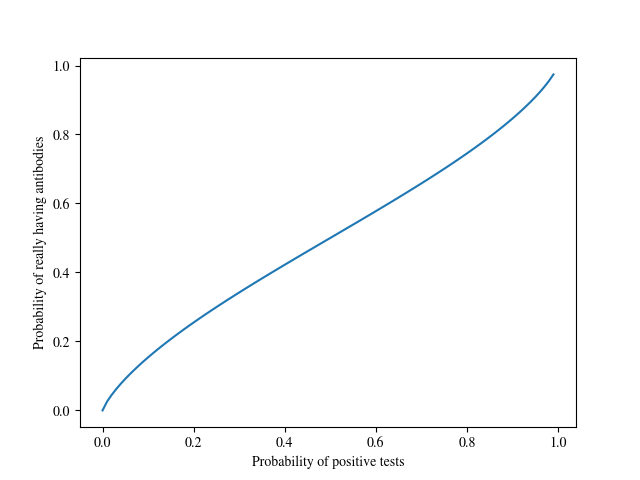
\includegraphics[width=\textwidth]{q2.png}
\end{figure}
